\documentclass[11pt]{article}
\usepackage[a4paper,margin=1in]{geometry}
\usepackage{amsmath, amssymb, amsthm}
\usepackage{booktabs}
\usepackage{graphicx}
\usepackage{csquotes}
\usepackage{float}
\usepackage[numbers,sort&compress]{natbib}

% TikZ and PGFPlots packages
\usepackage{tikz}
\usepackage{pgfplots}
\pgfplotsset{compat=1.18}

% Load 3D plotting libraries
\usetikzlibrary{arrows.meta}
\usetikzlibrary{decorations.markings}
\usetikzlibrary{calc}
\usetikzlibrary{positioning}

% PGFPlots 3D surface library
\usepgfplotslibrary{colormaps}
\usepgfplotslibrary{patchplots}


\title{Variance Reduction for Monte Carlo Pricing of Credit Derivatives}
\author{Olatomiwa Adewusi}
\date{October 19, 2025}

\begin{document}
\maketitle

\tableofcontents

% Option A: use \input so we don't create per-section .aux in build/
\section{Introduction}

This introduction outlines the project goals, constraints, and contribution. The project is a tutorial on Monte Carlo variance reduction with credit as an application domain. It motivates why stochastic hazards and exotic features push us to simulation, and it previews the toolkit and results.

\section{Literature Review}

\subsection{Scope, Motivation, and Related Literature}

Monte Carlo simulation is a central tool in computational finance and applied probability, particularly when analytical valuation becomes infeasible due to stochastic hazards or exotic payoff features. In credit derivatives, closed-form pricing breaks down once the hazard rate becomes stochastic or when coupons and redemptions depend on default outcomes. In such settings, Monte Carlo estimation provides a flexible numerical approach capable of handling discontinuities and complex path dependence. The challenge is not only to obtain unbiased estimators of expected payoffs but to do so efficiently by minimising variance for a fixed computational budget.

The methodological foundation of this project lies in the simulation and variance-reduction literature. \citet{lawKelton2015} provides the canonical reference on discrete-event and Monte Carlo simulation methodology, including estimator design, random-number generation, and efficiency-improvement techniques. \citet{glasserman2004} extends these ideas to financial engineering, offering rigorous treatments of convergence diagnostics, variance-reduction algorithms, and pathwise derivative estimation. Together they form the theoretical and algorithmic backbone of this work. 

The application context for this project draws on reduced-form credit modelling, where default is represented as a stochastic event governed by a hazard-rate process. \citet{schonbucher2003} presents a practitioner-oriented synthesis of intensity-based credit models and simulation approaches for credit derivatives, while \citet{okaneTurnbull2003} outlines the market conventions and bootstrapping techniques used to construct hazard curves and value credit default swaps (CDS). These texts provide the minimal domain knowledge required to translate generic Monte Carlo concepts into a credit-specific test case.

Beyond these four core references, broader treatments of credit risk appear in \citet{duffieSingleton2003}, \citet{lando2004}, and \citet{bieleckiRutkowski2002}, each formalising the mathematical foundations of intensity-based and structural models. \citet{brigoMercurio2006} complements these works by detailing interest-rate modelling and discounting frameworks relevant to credit-linked products. These additional sources are referenced for completeness but remain outside the primary simulation and variance-reduction focus of this project.

\subsection{Pseudo-Random Number Generation}

Monte Carlo methods depend on streams of pseudo-random numbers that emulate independent samples from the uniform distribution on $(0,1)$. Modern simulation packages typically use the Mersenne Twister algorithm \citep{matsumoto1998}, a 623-dimensionally equidistributed generator with an extremely long period of $2^{19937}-1$. NumPy, used in this project, adopts this generator by default. Each simulation uses an explicit seed to guarantee reproducibility, ensuring that all results are replicable. Because the Mersenne Twister already meets the quality criteria recommended by \citet{lawKelton2015}, no alternative generator is explored. The focus remains on how random draws are exploited within variance-reduction frameworks rather than on the mechanics of the generator itself.

\subsection{Monte Carlo Estimation and Error Analysis}

The standard Monte Carlo estimator for an expected value $\mu = \mathbb{E}[f(X)]$ is
\begin{equation}
    \hat{\mu}_N = \frac{1}{N}\sum_{i=1}^{N} f(X_i),
\end{equation}
where $X_i$ are independent random draws from the target distribution. By the Law of Large Numbers, $\hat{\mu}_N \rightarrow \mu$ almost surely as $N \rightarrow \infty$. The Central Limit Theorem implies
\begin{equation}
    \sqrt{N}(\hat{\mu}_N - \mu) \xrightarrow{d} \mathcal{N}(0, \sigma^2),
\end{equation}
so the standard error declines at rate $1/\sqrt{N}$. This slow convergence motivates the study of variance-reduction techniques that deliver comparable precision with fewer simulated paths \citep{glasserman2004, lawKelton2015}.

Error analysis decomposes mean-squared error into bias and variance. Since unbiased estimators have zero bias, simulation efficiency is governed mainly by variance. Empirical variance can be estimated via batch means or replication analysis, and confidence intervals quantify estimator precision. Figure~\ref{fig:mc-convergence} may illustrate the typical $1/\sqrt{N}$ convergence pattern.

\subsection{Variance Reduction Techniques}

Variance-reduction methods exploit structure in the problem to lower estimator variance without introducing bias. Let $\hat{\theta}$ denote a Monte Carlo estimator with variance $\mathrm{Var}[\hat{\theta}]$. A successful technique produces an alternative estimator $\hat{\theta}^{*}$ satisfying $\mathrm{Var}[\hat{\theta}^{*}] < \mathrm{Var}[\hat{\theta}]$ for equal computational effort.

\paragraph{Common Random Numbers (CRN).}
CRN reuses identical random-number streams across related simulations to induce positive correlation. If $Y_1$ and $Y_2$ are outputs using the same random seeds,
\[\mathrm{Var}(Y_1 - Y_2) = \mathrm{Var}(Y_1) + \mathrm{Var}(Y_2) - 2\rho\,\sigma_{Y_1}\sigma_{Y_2}.\]
A positive correlation $\rho$ lowers the variance of their difference, improving precision in comparative analyses such as sensitivity tests in credit simulations.

\paragraph{Antithetic Variates.}
Antithetic sampling generates negatively correlated pairs. For a uniform draw $U_i$, its complement $1-U_i$ provides an antithetic pair. When transformed via the Box–Muller or Polar method into standard normals, the resulting $(Z_i, -Z_i)$ pairs yield reduced estimator variance for monotonic payoffs \citep{glasserman2004}. The method is simple and typically effective.

\paragraph{Stratified and Latin Hypercube Sampling.}
Stratified sampling divides the uniform $(0,1)$ range into $K$ equal-probability strata, drawing one sample from each. The estimator becomes
\[\hat{\mu}_{strat} = \frac{1}{K}\sum_{i=1}^{K} f(F^{-1}(U_i)),\]
ensuring coverage across the distribution and reducing clustering in the tails. Latin Hypercube Sampling generalises this idea to multiple dimensions by enforcing stratification along each marginal. The design achieves superior space-filling and typically yields lower variance for smooth response surfaces \citep{lawKelton2015}. Figure~\ref{fig:lhs-schematic} can visualise the difference between random sampling and LHS.

\paragraph{Control Variates.}
Control variates exploit correlation with a secondary variable of known expectation. Given $f(X)$ and $g(X)$ with $\mathbb{E}[g(X)]$ known, the adjusted estimator is
\begin{equation}
    \hat{\mu}_{cv} = \bar{f} - b(\bar{g} - \mathbb{E}[g]),
\end{equation}
where $b^{*} = \mathrm{Cov}(f,g) / \mathrm{Var}(g)$. Variance reduction improves with correlation strength. In this project, an analytically priced risky bond serves as a control variate for the simulated credit-linked note payoff.

\subsection{Application to Credit Derivatives}

Credit derivatives provide a structured and intuitive test case for Monte Carlo simulation. A risky bond differs from a risk-free bond by the possibility of default, which halts coupon payments and triggers a recovery amount. A credit default swap transfers this risk: the buyer pays periodic premiums until default or maturity and receives compensation equal to the loss given default. The relationship
\[\text{Risk-Free Bond} = \text{Risky Bond} + \text{CDS}\]
captures this equivalence succinctly \citep{schonbucher2003}. A credit-linked note embeds this exposure in a funded form, offering higher coupons in exchange for assuming the reference entity’s default risk. In valuation terms, a CLN is a bond combined with a short CDS position \citep{okaneTurnbull2003}. Deterministic hazard frameworks derive survival from bootstrapped curves, while stochastic frameworks model the hazard as a random process requiring simulation. Variance-reduction methods enhance estimator stability in low-default regimes.

\subsection{Implementation and Practical Notes}

Simulations are implemented in Python using NumPy. The Mersenne Twister ensures reproducibility, and seeds are fixed for each experiment. Interest-rate and hazard-rate curves are represented by exponential functional forms for tractability. In production these curves would be bootstrapped from traded instruments such as swaps and CDSs, but that process lies outside this project’s scope. Calendar conventions and accrual adjustments are abstracted away, since the emphasis is on comparing convergence rates and variance-reduction performance rather than on reproducing full market infrastructure.

\subsection{Summary and Literature Gap}

While the literatures on Monte Carlo simulation and credit risk are individually mature, few studies apply variance-reduction methods systematically to credit-linked notes or related structures. This project fills that gap by demonstrating how classical techniques can improve estimator precision for stochastic-hazard credit payoffs.

\section{Credit Model Setup}

\subsection{Credit Product Definitions}

This section introduces three core instruments used throughout the project: risky bonds, credit default swaps, and credit linked notes. The goal is to give a clear, intuitive explanation that assumes no prior knowledge of credit markets. We first explain how default works, then show how discount factors and survival probabilities enter the valuation of each cashflow. We break each payoff into simple components and give diagrams that illustrate the structure visually.

\subsubsection*{Default, Recovery, and Survival}

A borrower may default at any time before a bond matures. Default means:
\begin{itemize}
    \item all future coupon payments stop,
    \item the principal is not paid back in full,
    \item instead the investor receives a recovery amount $R$ times notional,
    \item recovery is typically paid immediately when default occurs.
\end{itemize}

If default happens at time $t$, this event has probability density $h(t) Q(0,t)$, where $h(t)$ is the hazard rate and $Q(0,t)$ is the survival probability up to $t$. This explains why recovery terms appear as integrals whereas coupons appear as summations over discrete dates.

Discount factors $P(0,t)$ reduce future cashflows to present value. Survival probabilities $Q(0,t)$ weigh cashflows by the chance that the issuer has not defaulted.

\subsubsection*{Risky Bonds}

A risky bond pays periodic coupons and a principal at maturity, but only if the issuer survives until these dates. If the issuer defaults earlier, coupons stop and the investor receives a recovery payment. We decompose the value of a risky bond into three parts:

\paragraph{1. Coupon leg}
\[
V_{\text{coupon}} = \sum_{i} c\,P(0,t_i)\,Q(0,t_i).
\]

\paragraph{2. Redemption leg}
\[
V_{\text{redemption}} = P(0,T)\,Q(0,T).
\]

\paragraph{3. Recovery leg}
\[
V_{\text{recovery}}
= \int_0^T R\,P(0,t)\,h(t)\,Q(0,t)\,dt.
\]

\paragraph{Total value}
\[
V_{\text{risky}} = V_{\text{coupon}} + V_{\text{redemption}} + V_{\text{recovery}}.
\]

\paragraph{Cashflow diagram}

\begin{verbatim}
Time:   0         t1        t2        ...       T
        |---------|---------|---------|---------|
Cash:     c        c         c         c     +1 (if survive)
Default:           X  ---> Recovery R * Notional
\end{verbatim}

\subsubsection*{Credit Default Swaps}

A credit default swap (CDS) transfers the default risk of a reference entity from one party to another. There are two legs.

\paragraph{1. Premium leg}
\[
V_{\text{prem}} = s \sum_{i} P(0,t_i)\,Q(0,t_i).
\]

\paragraph{2. Protection leg}
\[
V_{\text{prot}} = (1-R)\int_0^T P(0,t)\,h(t)\,Q(0,t)\,dt.
\]

\paragraph{Fair spread}
\[
V_{\text{prem}} = V_{\text{prot}}.
\]

\paragraph{Intuition}
\begin{itemize}
    \item A protection buyer is short credit risk.
    \item A protection seller is long credit risk.
\end{itemize}

\subsubsection*{Identity Linking Bonds and CDS}

\[
\text{Risk Free Bond} = \text{Risky Bond} + \text{CDS}.
\]

This identity shows how the CDS removes the risky bond’s default component.

\subsubsection*{Credit Linked Notes}

A credit linked note embeds a short CDS position into a funded bond:
\[
\text{CLN} = \text{Risk Free Bond} - \text{CDS}.
\]

The coupon is higher because the investor is selling credit protection. CLNs allow institutions that cannot trade derivatives to take credit risk in a funded format.

% =======================================================================
% DETERMINISTIC CURVES
% =======================================================================

\subsection{Deterministic Hazard and Short Rate Curves}

Default risk is represented through a hazard rate $h(t)$, giving survival
\[
Q(0,t) = \exp\left(-\int_0^t h(u)\,du\right).
\]
Similarly,
\[
P(0,t) = \exp\left(-\int_0^t r(u)\,du\right)
\]
gives discounting.

We avoid market calibration and instead specify smooth parametric curves with closed-form integrals.

\subsection{Exponential Hazard and Short Rate Curves}

\[
r(t) = a_r + b_r e^{-c_r t}, \qquad
h(t) = a_h + b_h e^{-c_h t}.
\]

Integrated forms:
\[
Q(0,t) = \exp\Big(-a_r t - \frac{b_r}{c_r}(1 - e^{-c_r t})\Big),
\]
\[
S(0,t) = \exp\Big(-a_h t - \frac{b_h}{c_h}(1 - e^{-c_h t})\Big).
\]

These deterministic curves will become the \textit{initial conditions} for the HJM model.

\subsection{Interpretation of the Parameters}

\paragraph{Long-run level $a$} sets the asymptotic intensity/rate.  
\paragraph{Shift $b$} controls slope at $t=0$.  
\paragraph{Speed $c$} determines exponential decay, equivalently the half-life:
\[
t_{1/2} = \frac{\ln 2}{c}.
\]

\subsection{Chosen Parameters and Economic Motivation}

The project uses simple but realistic parameter sets for the short rate and for two credit qualities: an investment grade (IG) name and a high yield (HY) name. These curves are chosen for plausibility rather than calibration but retain appropriate risk levels and term structure slopes.

\paragraph{Short rate parameters}
\begin{align*}
a_r = 0.02, \qquad b_r = 0.02, \qquad c_r = 0.35.
\end{align*}
This yields $r(0) = 4\%$ and a long run level of $2\%$. The half life is approximately two years. This generates a mild downward slope that is consistent with many developed market environments.

\paragraph{Investment grade hazard rate}
\begin{align*}
a_h = 0.015, \qquad b_h = -0.012, \qquad c_h = 0.30.
\end{align*}
This gives $h(0) = 0.003$ and a long run intensity of $0.015$. The curve slopes upward with a half life near 2.3 years. This matches the pattern of IG credit risk where short horizon default risk is very small but long run uncertainty is higher.

\paragraph{High yield hazard rate}
\begin{align*}
a_h = 0.03, \qquad b_h = -0.02, \qquad c_h = 0.40.
\end{align*}
This yields $h(0) = 0.01$ and a long run intensity of $0.03$. The slope is steeper and the half life is shorter (about 1.7 years). This reflects the behaviour of BB or B rated credits with materially higher default risk.

\subsection{Spread Interpretation Under Recovery}

Under reduced form modelling with recovery of par, the credit spread associated with a hazard rate is
\begin{equation}
s(t) = (1 - R)\,h(t),
\end{equation}
and we adopt $R = 40\%$ which is standard for unsecured corporates.

\paragraph{Investment grade spreads}
\begin{align*}
s_{\text{IG}}(0) &= 0.6 \times 0.003 = 18\ \text{bps}, \\
s_{\text{IG}}(\infty) &= 0.6 \times 0.015 = 90\ \text{bps}.
\end{align*}

\paragraph{High yield spreads}
\begin{align*}
s_{\text{HY}}(0) &= 0.6 \times 0.01 = 60\ \text{bps}, \\
s_{\text{HY}}(\infty) &= 0.6 \times 0.03 = 180\ \text{bps}.
\end{align*}

These spread levels are reasonable for IG and HY credit and support the qualitative interpretation of the chosen parameters.


% =======================================================================
% HJM FRAMEWORK
% =======================================================================

\subsection{HJM Framework for Rates and Hazards}

The deterministic short rate curve $r(t)$ and hazard rate curve $h(t)$ provide the initial term structures of discount and survival. The Heath–Jarrow–Morton (HJM) approach takes these initial curves as inputs and specifies arbitrage-free stochastic dynamics for the entire forward curve. In HJM models the forward curve is the fundamental state variable and all randomness enters through its evolution rather than through the initial term structure.

\subsubsection*{Short Rate, Forward Rate, and Their Relationships}

The short rate $r(t)$ represents the instantaneous risk-neutral interest rate at time $t$. The price of a zero-coupon bond maturing at $T$ is
\[
P(t,T) = \mathbb{E}_t\left[\exp\Big(-\int_t^T r_u \, du\Big)\right].
\]

The instantaneous forward rate $f(t,T)$ is defined by
\[
f(t,T) = -\frac{\partial}{\partial T}\log P(t,T),
\]
which represents the rate applied over an infinitesimal period at time $T$. The short rate is recovered from the diagonal:
\[
r_t = f(t,t).
\]

When $r(t)$ is deterministic,
\[
P(0,T) = \exp\Big(-\int_0^T r(u)\,du\Big),
\qquad
f(0,T) = r(T).
\]
Thus the deterministic short rate curve is equal to the initial forward curve.

\subsubsection*{Hazard Rate, Forward Hazard, and Their Relationships}

The hazard rate $h(t)$ is the instantaneous default intensity. Survival to $T$ is
\[
Q(t,T) = \mathbb{E}_t\left[\exp\Big(-\int_t^T h_u \, du\Big)\right].
\]

The forward hazard rate is
\[
\gamma(t,T) = -\frac{\partial}{\partial T}\log Q(t,T),
\qquad
h_t = \gamma(t,t).
\]

In the deterministic case,
\[
Q(0,T) = \exp\Big(-\int_0^T h(u)\,du\Big),
\qquad
\gamma(0,T) = h(T).
\]
The deterministic hazard curve is therefore the initial forward hazard surface.

\subsubsection*{Initial Forward Surfaces for HJM}

The exponential deterministic curves derived earlier give
\[
f(0,T) = r(T),
\qquad
\gamma(0,T) = h(T).
\]
These surfaces serve as the initial conditions for the HJM evolution.

\subsubsection*{HJM Dynamics and Drift Conditions}

HJM specifies forward dynamics of the form
\[
df(t,T) = \alpha_r(t,T)\,dt + \sigma_r(t,T)\,dW^{(r)}_t,
\]
\[
d\gamma(t,T) = \alpha_h(t,T)\,dt + \sigma_h(t,T)\,dW^{(h)}_t,
\]
with instantaneous correlation
\[
dW^{(r)}_t dW^{(h)}_t = \rho\,dt.
\]

We adopt one-factor exponential volatilities,
\[
\sigma_r(t,T) = \sigma_r e^{-c_r (T-t)},
\qquad
\sigma_h(t,T) = \sigma_h e^{-c_h (T-t)}.
\]

The HJM drift restriction ensures absence of arbitrage. It gives
\[
\alpha_r(t,T) 
= \sigma_r(t,T)\int_t^T \sigma_r(t,s)\,ds
= \frac{\sigma_r^2}{2c_r}\big(1 - e^{-2c_r (T-t)}\big),
\]
\[
\alpha_h(t,T) 
= \sigma_h(t,T)\int_t^T \sigma_h(t,s)\,ds
= \frac{\sigma_h^2}{2c_h}\big(1 - e^{-2c_h (T-t)}\big).
\]

Forward surfaces evolve as
\[
f(t,T) = f(0,T) + \int_0^t \alpha_r(u,T)\,du 
+ \int_0^t \sigma_r(u,T)\,dW^{(r)}_u,
\]
\[
\gamma(t,T) = \gamma(0,T) + \int_0^t \alpha_h(u,T)\,du 
+ \int_0^t \sigma_h(u,T)\,dW^{(h)}_u.
\]

\subsubsection*{Interpretation of Forward Curve Evolution}

The HJM framework models the time evolution of the entire forward curve. The forward rate $f(t,T)$ is defined for maturities $T \ge t$, and at each observation time $t$ the function $T \mapsto f(t,T)$ describes the market-implied instantaneous rates for all remaining maturities. As time increases, both the domain and the shape of this forward curve change.

At time $0$ the full forward curve
\[
f(0,T), \qquad T \in [0,T^*],
\]
is observable from the initial term structure. This curve represents the market-implied future short rates from the present time.

At a later time $t_1$ one observes a new forward curve
\[
f(t_1,T), \qquad T \ge t_1.
\]
The portion of the original curve with maturities $T < t_1$ is no longer relevant because those maturities lie in the past. The short rate at time $t_1$ is obtained from the diagonal through
\[
r(t_1) = f(t_1,t_1).
\]

At a later time $t_2$ the entire curve evolves again,
\[
f(t_2,T), \qquad T \ge t_2,
\]
and both its location and its shape change due to the stochastic HJM dynamics. The curve now begins at the point $T = t_2$, and its behaviour for $T > t_2$ reflects the accumulated randomness up to time $t_2$.

This picture highlights several key properties that are central to HJM modelling.

\begin{figure}[H]
\centering
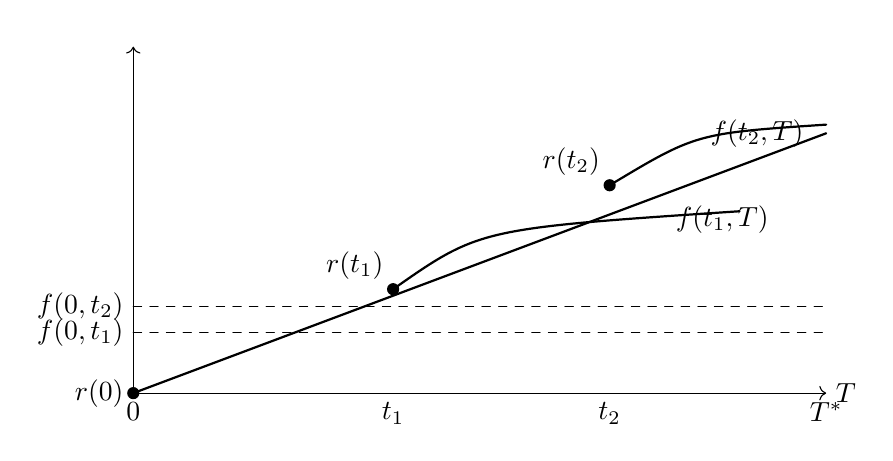
\begin{tikzpicture}[scale=1.1, line cap=round, line join=round]

% Axes
\draw[->] (0,0) -- (8,0) node[right] {$T$};
\draw[->] (0,0) -- (0,4) node[above] {};

% Labels on T-axis
\node[below] at (0,0) {$0$};
\node[below] at (3,0) {$t_1$};
\node[below] at (5.5,0) {$t_2$};
\node[below] at (8,0) {$T^*$};

% Short rate points on diagonal
\draw[thick] (0,0) -- (8,3);

\fill (0,0) circle (2pt);
\fill (3,1.2) circle (2pt);
\fill (5.5,2.4) circle (2pt);

\node[left] at (0,0) {$r(0)$};
\node[above left] at (3,1.2) {$r(t_1)$};
\node[above left] at (5.5,2.4) {$r(t_2)$};

% Forward curve f(0,T) at time 0 (flat dashed)
\draw[dashed] (0,1) -- (8,1);
\node[left] at (0,1) {$f(0,t_2)$};

\draw[dashed] (0,0.7) -- (8,0.7);
\node[left] at (0,0.7) {$f(0,t_1)$};

% Forward curve at time t1
\draw[thick] (3,1.2) .. controls (4,1.9) .. (7,2.1);

% Forward curve at time t2
\draw[thick] (5.5,2.4) .. controls (6.5,3.0) .. (8,3.1);

% Labels for forward curves
\node at (6.8,2.0) {$f(t_1,T)$};
\node at (7.2,3.0) {$f(t_2,T)$};

\end{tikzpicture}
\caption{Evolution of the forward curve. At time zero, the forward curve
$f(0,T)$ is defined for maturities in $[0,T^*]$ and the short rate is $r(0)=f(0,0)$.
At time $t_1$ the forward curve $f(t_1,T)$ is defined for maturities in
$[t_1,T^*]$, and the short rate is $r(t_1)=f(t_1,t_1)$.}
\end{figure}

\begin{itemize}
    \item The forward curve evolves as a random function. At times $t_0$, $t_1$, and $t_2$ the entire mapping $T \mapsto f(t,T)$ shifts according to the dynamics implied by the forward SDE.
    \item The short rate always lies on the diagonal $T = t$ and satisfies $r(t) = f(t,t)$. This identity is fundamental because the short rate drives discounting and appears in all risk-neutral valuation formulas.
    \item As time increases, the region $T < t$ becomes irrelevant. The forward curve is only defined for maturities that remain in the future relative to the current time.
    \item HJM models the full forward curve rather than the short rate. The short rate is recovered from the diagonal, but the dynamics are specified for the entire surface $f(t,T)$.
    \item The simulated object in a Monte Carlo implementation is therefore a curve-valued stochastic process. For every simulation path and every time step, one obtains a full forward curve $f(t,T)$ for all $T \ge t$.
\end{itemize}

These ideas extend directly to the forward hazard surface $\gamma(t,T)$ used for credit modelling. In the CLN valuation framework the HJM dynamics generate stochastic forward hazard curves. At each time step the instantaneous hazard rate is extracted from the diagonal through
\[
h_t = \gamma(t,t),
\]
and this quantity drives CDS spreads, survival probabilities, barrier conditions, optional redemptions, and any payoff components that depend on credit quality. Forward hazard evolution ensures that the expected survival curve matches the deterministic initial curve, which is essential for unbiased Monte Carlo pricing.

Understanding the evolution of the forward surfaces $f(t,T)$ and $\gamma(t,T)$ clarifies the structure of the simulation. It explains why diagonals determine the instantaneous rates, why pathwise integrals of these rates appear in discount and survival factors, and how deterministic term structures propagate consistently into stochastic valuation. This conceptual view forms the link between deterministic credit curves, stochastic forward hazard modelling, and the pathwise hazard rates used in credit-linked note pricing.


\subsubsection*{Bond Prices, Survival, and Instantaneous Rates}

The HJM evolution provides the entire forward surfaces $f(t,T)$ and $\gamma(t,T)$ for interest rates and hazard rates. From these surfaces we recover bond prices, survival probabilities, and the instantaneous short rate and spot hazard rate. These quantities are needed for Monte Carlo valuation of credit-linked notes.

\paragraph{Recovering bond prices and survival probabilities.}

Given forward surfaces at time $t$, the pathwise zero-coupon bond price and survival value are
\[
P(t,T) = \exp\Big(-\int_t^T f(t,u)\,du\Big),
\qquad
Q(t,T) = \exp\Big(-\int_t^T \gamma(t,u)\,du\Big).
\]
These identities hold in both deterministic and stochastic settings. The HJM drift restriction ensures
\[
\mathbb{E}\left[P(t,T)\right] = P(0,T),
\qquad
\mathbb{E}\left[Q(t,T)\right] = Q(0,T),
\]
which guarantees that the simulated curves reproduce the initial term structures in expectation.

\paragraph{Instantaneous rates along the path}

The short rate and spot hazard rate are obtained from the diagonals:
\[
r_t = f(t,t),
\qquad
h_t = \gamma(t,t).
\]
Since negative hazard rates are not meaningful, we apply
\[
h_t \leftarrow \max\{h_t, 0\}.
\]
The accumulated discount factor and survival factor along a simulation path are
\[
D(0,t) = \exp\Big(-\int_0^t r_u\,du\Big),
\qquad
S(0,t) = \exp\Big(-\int_0^t h_u\,du\Big).
\]

\paragraph{Why the pathwise integrals are required.}

Many exotic credit products depend on the instantaneous hazard rate or the cumulative hazard along the path. For example, model-implied CDS spreads satisfy
\[
s_t = (1 - R)\,h_t,
\]
so any payoff referencing credit spreads must use the simulated $h_t$ at each step. Callable and barrier CLNs may depend on the survival value $Q(t,T)$ or on the mark-to-market spread at call dates. Range accrual CLNs often require the hazard rate to remain inside or outside a region.

Even when a payoff depends only on credit quantities, the risk-neutral valuation formula requires discounting through
\[
D(0,t) = \exp\Big(-\int_0^t r_u\,du\Big),
\]
so the short rate must also be accumulated along the path.

\paragraph{Role of the forward SDEs in simulation.}

The forward dynamics
\[
df(t,T) = \alpha_r(t,T)\,dt + \sigma_r(t,T)\,dW^{(r)}_t,
\qquad
d\gamma(t,T) = \alpha_h(t,T)\,dt + \sigma_h(t,T)\,dW^{(h)}_t,
\]
are discretised in time in the Monte Carlo simulation. At each step the entire forward curve is updated, and the diagonal values $r_t = f(t,t)$ and $h_t = \gamma(t,t)$ are extracted. Numerical integration of these processes yields $D(0,t)$ and $S(0,t)$, which drive the pricing of all subsequent CLN cashflows.

The implementation details, including discretisation schemes and variance reduction, are presented in the following section.


% =======================================================================
% HJM MONTE CARLO IMPLEMENTATION (HAZARD RATES)
% =======================================================================

\section{Monte Carlo Implementation of the HJM Hazard Model}

\paragraph{Note on Sources.}
The Monte Carlo formulation in this section follows the structure of 
\cite{glasserman2004} \textit{Monte Carlo Methods in Financial Engineering} 
, Chapter~3, and in particular Sections~3.6 and~3.6.1.  
The original presentation concerns interest-rate term-structure models, 
and has been translated here into the credit-risk setting.  
The notation has been adjusted, but the foundations are based on Glasserman's work.

The previous subsection introduced the continuous time HJM framework for
forward hazard rates $\gamma(t,T)$ and showed how it preserves today’s survival
curve $S(0,T)$ in expectation. We now translate that theory into a concrete
Monte Carlo recipe that can be coded directly.

The guiding principles are the same as in the classical HJM interest rate
literature, but applied to credit:

\begin{itemize}
    \item Work with the \emph{forward hazard surface} $\gamma(t,T)$, not directly
          with $h(t)$.
    \item Initialise a \emph{discrete} forward hazard surface so that it matches
          the deterministic survival curve exactly on the simulation grid.
    \item Evolve the surface in time using a one factor volatility structure and
          a discrete drift chosen to keep survival probabilities arbitrage free
          on the grid.
    \item Read the diagonal to obtain the instantaneous hazard $h(t)$ along each
          path, then integrate $h(t)$ to obtain survival factors and default
          times.
\end{itemize}

Throughout this section we keep the short rate deterministic, so all discount
factors $D(0,t)$ can be precomputed and taken outside the simulation. The Monte
Carlo part of the model carries only \emph{credit} randomness. 

\subsection{Time and Maturity Grids}

We use a single time grid for both simulation time and credit maturities:
\[
0 = t_0 < t_1 < \dots < t_N = T_{\max},
\qquad
\Delta t_i = t_{i+1} - t_i.
\]

In practice:

\begin{itemize}
    \item Choose $T_{\max}$ to be at least the final maturity of all instruments
          in the portfolio.
    \item Use a relatively fine grid around coupon dates and potential call or
          knock out dates, and a coarser grid in between.
    \item For simplicity we let both arguments of $\gamma$ live on this same
          grid, so we will approximate $\gamma(t_i, T_j)$ only for $0 \le i \le j
          \le N$.
\end{itemize}

We denote the discrete approximation by $\widehat{\gamma}(t_i, t_j)$, or more
compactly by $\gamma_{i,j}$ when the meaning is clear.

\subsection{Precomputation of the Deterministic Survival and Discount Curves}

From the parametric curves $r(t)$ and $h(t)$ we compute

\[
D(0,t)
  = \exp\!\left(-\int_0^t r(u)\,du\right), 
\qquad
S(0,t)
  = \exp\!\left(-\int_0^t h(u)\,du\right),
\]

for all grid points $t = t_0,\dots,t_N$. These integrals are closed form for the
exponential specifications used in this project, so this step is analytic and
cheap.

\begin{itemize}
    \item The discount factors $D(0,t_i)$ will be used only for present valuing
          cashflows and do not interact with the Monte Carlo evolution.
    \item The survival probabilities $S(0,t_i)$ will be used to initialise the
          forward hazard surface in a way that is exactly consistent with the
          deterministic curve.
\end{itemize}

\subsection{Discrete Initial Forward Hazard Surface}

In continuous time the relationship between the forward hazard curve and the
survival function at time $t$ is
\[
S(t,T)
  = \exp\!\left(-\int_t^T \gamma(t,u)\,du\right).
\]

On the discrete grid we approximate this by
\[
\widehat{S}(t_i, t_j)
  = \exp\!\left(-\sum_{l=i}^{j-1} \gamma_{i,l}\,\Delta t_l\right),
  \qquad j > i,
\]
with the convention $\widehat{S}(t_i, t_i) = 1$.

To ensure that the simulated model exactly matches the deterministic survival
curve at $t = 0$ we demand
\[
\widehat{S}(0, t_j) = S(0, t_j),
\qquad j = 0,\dots,N.
\]
This leads to the recursion
\[
\widehat{S}(0, t_{j+1})
 = \widehat{S}(0, t_j)
   \exp\!\left(-\gamma_{0,j}\,\Delta t_j\right),
\]
hence
\[
\gamma_{0,j}
  = -\frac{1}{\Delta t_j}
     \log\frac{S(0, t_{j+1})}{S(0, t_j)},
  \qquad j = 0,\dots,N-1.
\]

\paragraph{Interpretation}
The discrete forward hazard $\gamma_{0,j}$ is the \emph{average} of the
continuous forward hazard over $[t_j,t_{j+1}]$. Directly sampling
$\gamma(0,t_j)$ from the continuous formula would not preserve the survival
curve on the grid. Matching the log ratio
$S(0,t_{j+1})/S(0,t_j)$ is therefore essential.

\subsection{Discretising the Volatility Surface}

The continuous model specifies a one factor exponential volatility structure
\[
\sigma_h(t,T) = \sigma_h\, e^{-c_h(T - t)}.
\]
On the discrete grid we simply sample this at the grid points:
\[
\widehat{\sigma}_h(t_i, t_j)
  = \sigma_h\, e^{-c_h(t_j - t_i)},
  \qquad j \ge i.
\]

For simulation it is convenient to write
\[
\sigma_{i,j} := \widehat{\sigma}_h(t_i, t_j),
\]
and to use a single scalar Brownian motion per path.

\subsection{Discretising HJM Drift on the Grid}

In continuous time the HJM drift restriction ensures that survival curves
remain arbitrage free. On the discrete grid we want an analogous property:
for each maturity $T_j$ the survival value $S(t_i, t_j)$ should evolve as a
martingale when discounted appropriately.

The standard HJM trick is to construct the discrete drift from the volatility
surface directly. In style of \cite{glasserman2004} (Specifically 3.6.2, The discrete drift), define for fixed $i$ the cumulative
volatility weights
\[
w_n
  = \sum_{l=i}^n \sigma_{i-1,l}\,\Delta t_l,
  \qquad n = i,\dots,N-1,
\]
with $w_{i-1} := 0$.

The arbitrage free discrete drift at time step $t_{i-1} \to t_i$ is then given by
\[
\widehat{\alpha}_h(t_{i-1}, t_j)
  = \mu_{i-1,j}
  = \frac{w_j^2 - w_{i-1}^2}{2\,\Delta t_j},
  \qquad j = i,\dots,N-1.
\]

This is the exact discrete counterpart of the continuous time HJM drift
condition. It ensures that the discrete survival curve implied by
$\gamma_{i,\cdot}$ is consistent with no arbitrage on the grid.

\paragraph{Important warning.}
A naive Euler discretisation of
\[
d\gamma(t,T) = \alpha_h(t,T)\,dt + \sigma_h(t,T)\,dW_t
\]
at each maturity $T$ separately breaks the discrete martingale property and
causes slow drift in the survival curve as $i$ increases. The construction
above explicitly couples all maturities through the cumulative weights $w_n$
and avoids this problem.

\subsection{Forward Hazard Update per Time Step}

Given $\gamma_{i-1,j}$ for $j \ge i-1$ at time $t_{i-1}$ we update the forward
hazards to $t_i$ as follows.

\begin{enumerate}
    \item Compute the volatility slice
          \[
          \sigma_{i-1,j} = \sigma_h\, e^{-c_h(t_j - t_{i-1})},
          \qquad j = i,\dots,N-1.
          \]
    \item Form the cumulative volatility weights
          \[
          w_n
            = \sum_{l=i}^n \sigma_{i-1,l}\,\Delta t_l,
            \qquad n = i,\dots,N-1,
          \]
          and set $w_{i-1} = 0$.
    \item Compute the discrete drift
          \[
          \mu_{i-1,j}
            = \frac{w_j^2 - w_{j-1}^2}{2\,\Delta t_j},
            \qquad j = i,\dots,N-1.
          \]
    \item Draw a single standard normal $Z_i \sim \mathcal{N}(0,1)$ for this
          time step.
    \item Update the forward hazards
          \[
          \gamma_{i,j}
            = \gamma_{i-1,j}
              + \mu_{i-1,j}\,\Delta t_{i-1}
              + \sigma_{i-1,j}\,\sqrt{\Delta t_{i-1}}\,Z_i,
            \qquad j = i,\dots,N-1.
          \]
\end{enumerate}

Values with $j < i$ correspond to maturities that have already passed, so they
are no longer part of the forward surface.

% =======================================================================
% 3.7  Pathwise Survival Under HJM Hazard Dynamics
% =======================================================================

\subsection{Pathwise Survival Under HJM Hazard Dynamics}

In many reduced-form credit models, default times are simulated explicitly by
drawing an exponential random variable and comparing it with the integrated
hazard process. While this method is theoretically correct, it produces
\emph{discontinuous} payoff behaviour across paths: cashflows abruptly drop to
zero once a simulated default time, $\tau$, falls before maturity. For instruments
with embedded optionality (e.g.  callable coupon structures, range-accrual
credit-linked notes, and digital redemption features) this “hard default” logic
leads to numerical kinks and unstable Monte Carlo convergence.

In this project we instead adopt a \emph{pathwise survival weighting} approach.
Rather than simulating default times, each Monte Carlo path produces a
\emph{forward hazard surface}
\[
\gamma_{i,j} := \widehat{\gamma}(t_i, t_j),
\qquad j \ge i,
\]
from which a full pathwise survival curve is constructed.

Given the forward hazards at simulation time $t_i$, the model-implied survival
from $t_i$ to $t_j$ is
\[
S(t_i, t_j)
    = \exp\!\left(
        - \sum_{\ell=i}^{j-1}
           \gamma_{i,l}\,\Delta t_\ell
      \right).
\]

This expression is evaluated \emph{on every path}. Consequently:

\begin{itemize}
    \item No default time is drawn.
    \item No cashflow is ever forcibly set to zero.
    \item All valuation is performed under smooth, differentiable
          survival weights $S(t_i,t_j)\in(0,1]$.
\end{itemize}

For each Monte Carlo path $p$, the contribution of a cashflow $c_j$ payable at
$t_j$ is
\[
\mathrm{PV}^{(p)}(c_j)
    = D(0,t_j)\,c_j\,S^{(p)}(t_i, t_j).
\]
Averaging over paths yields an unbiased Monte Carlo estimator of the true
reduced-form value. As we will see later, this smooth
treatment of survival probability is essential for structured CLN features,
ensuring stable simulation behaviour and eliminating numerical discontinuities.


% =======================================================================
% 3.8  From Forward Hazards to Instantaneous Hazard and Model CDS Levels
% =======================================================================

\subsection{From Forward Hazards to Instantaneous Hazard and Model CDS Levels}

As described in the previous chapter, the HJM hazard model evolves the \emph{forward hazard surface}
$\gamma(t,T)$ across simulation time. The instantaneous hazard rate at
time $t_i$ is obtained from the diagonal of this surface,
\[
h_i = \gamma_{i,i}.
\]
This instantaneous intensity determines the short-term default risk on
each Monte Carlo path.

For exotic credit-linked notes, coupons or
embedded options are often linked to the prevailing level of credit
risk, typically expressed in terms of a CDS spread. In a full
market-accurate implementation, the par CDS spread would be computed
using protection and premium leg present values, accounting for
discounting, accrual on default, payment conventions, and the term
structure of survival probabilities.

Such detail is unnecessary for the numerical experiments in this
tutorial. Instead, the \emph{model CDS spread} at time $t_i$ is defined
pathwise by
\[
s_i := (1 - R)\,h_i = (1 - R)\,\gamma_{i,i}.
\]

This quantity serves as the credit-risk state variable inside CLN
payoffs. All CDS-linked features are evaluated using
$s_i$. Since $h_i$ depends smoothly on the evolved forward hazards, the
resulting model CDS level reacts smoothly to volatility and curve
shifts, ensuring stable Monte Carlo behaviour.

\subsubsection*{Remark on Modelling Choice}

This simplified approach is appropriate here because the focus of the
tutorial is on the Monte Carlo implementation of the HJM hazard model,
rather than on exact replication of market CDS conventions. Should a
more realistic CDS calibration be required, the same forward-hazard
paths may be used to compute par spreads using full survival-based
leg valuations. That extension is conceptually straightforward but adds
substantial notational overhead without affecting the numerical
principles developed in this section.


\subsection{Exotic Range--Accrual CLN Payoff}

This section introduces the exotic payoff used throughout Chapter~4 to illustrate
variance--reduction methods. The product is a range--accrual credit--linked note
in which the final redemption amount is scaled by the proportion of
coupon--observation dates on which the model--implied CDS spread stays inside a
fixed corridor. The structure preserves the standard coupon, recovery, and
redemption legs of a risky bond while introducing controlled path dependence.

Let $t_1,\dots,t_N$ denote the coupon observation dates. Along each simulated
hazard--rate path, the HJM model produces a model--implied CDS spread $s(t_i)$.
Fix a corridor $[L,U]$ and define
\[
I_i = 1\{L \le s(t_i) \le U\},
\qquad
A = \frac{1}{N}\sum_{i=1}^N I_i.
\]
The factor $A$ measures the fraction of times the spread remains within the
corridor. At maturity, the notional is scaled by this factor, producing a smooth
and intuitive form of path dependency.

Let $D(0,t)$ and $S(0,t)$ denote the pathwise discount factor and pathwise
survival probability along the simulated hazard--rate path.

\subsubsection*{Coupon Leg}

The coupon leg follows the standard reduced--form representation:
\[
\text{CouponLeg}
= \sum_{i=1}^N c\, D(0,t_i)\, S(0,t_i),
\]
where $c$ is the contractual coupon. No exotic modification is applied to this
component.

\subsubsection*{Recovery Leg}

In reduced--form credit models, default can occur at any time, and its timing is
governed by the hazard rate $h(t)$. The key quantity is the \emph{default
density},
\[
h(t)\, S(0,t)\, dt,
\]
which represents the probability of default in the small interval around $t$.
Multiplying this by the recovery amount $R$ and the discount factor $D(0,t)$
gives the time--$t$ contribution of recovery to the overall price. In continuous
time, the recovery leg is
\[
\text{RecoveryLeg}
= R \int_0^T D(0,t)\, h(t) S(0,t)\, dt.
\]

For implementation, this integral is approximated on the same grid used for
coupon dates and survival simulation. This maintains conceptual clarity, avoids
the need for finer quadrature, and is adequate for the pedagogical and
variance--reduction focus of this project.

A convenient discrete approximation, which avoids evaluating $h(t)$ directly,
uses the identity
\[
h(u_j)\, S(0,u_j)\, \Delta u_j
\approx S(0,u_{j-1}) - S(0,u_j),
\]
expressing default over the interval $[u_{j-1},u_j]$ purely in terms of survival
probabilities. On the grid $0 = u_0 < u_1 < \dots < u_N = T$, the recovery leg
is therefore
\[
\text{RecoveryLeg}
= R \sum_{j=1}^{N} D(0,u_j)\, \bigl(S(0,u_{j-1}) - S(0,u_j)\bigr).
\]

\subsubsection*{Redemption Leg}

Only the redemption amount is affected by the range--accrual feature. Instead of
paying the full notional at maturity, the product pays
\[
\text{RedemptionLeg}
= A \cdot \mathrm{Notional} \cdot D(0,T)\, S(0,T).
\]
If the CDS spread is always inside the corridor, $A = 1$ and the standard CLN
redemption is recovered; if it spends significant time outside the corridor, the
redemption amount is proportionally reduced.

\subsubsection*{Full Exotic Payoff}

Combining all components, the payoff for a single Monte Carlo path is
\[
\text{Payoff}
= \text{CouponLeg}
+ \text{RecoveryLeg}
+ \text{RedemptionLeg}.
\]

This formulation maintains the classical risky--bond decomposition while
introducing a smooth and interpretable path--dependent element. Because the
exotic modification interacts closely with the vanilla CLN structure but varies
nonlinearly with spread dynamics, it serves as an ideal payoff for demonstrating
the effect of common random numbers, control variates, and antithetic variates.

This completes the numerical cookbook for the HJM hazard model. The next section will discuss variance reduction 
techniques in detail. 
\section{Numerical Experiments and Results}

Present quantitative comparisons, variance reduction factors, and convergence plots for the techniques across toy problems and credit payoffs.

\section{Discussion of Results}

Interpret the results. Explain when each method performs well or poorly. Discuss correlation strength for control variates and monotonicity for antithetic.

\section{Exotic Extensions}

Outline conceptual extensions such as range accrual features or multi-factor hazard models. Keep scope conceptual.

\section{Implementation Notes}

\subsection{Environment and Dependencies}

List Python and NumPy versions, Matplotlib, and any other packages. State the fixed RNG seed.

\subsection{Reproducibility Recipe}

Give a step-by-step recipe to reproduce results: set seed, generate uniforms, transform variates, run estimators, record CIs, and plot funnels. Avoid long code listings.

\section{Conclusion}

This project was both challenging and rewarding. I had prior exposure to quantitative finance, but credit derivatives were new to me, so building everything from first principles was a significant learning experience. Working through reduced–form credit modelling, hazard rates, and the HJM framework gave me a much clearer understanding of how credit term structures behave and how they feed into pricing.

A major part of the project involved implementing complex payoff logic in Python. The range–accrual CLN required careful structuring of the simulation code and forced me to think clearly about discounting, survival weighting, recovery modelling, and pathwise state variables such as CDS spreads. Writing all of this from scratch was difficult, but it made the numerical experiments feel much more meaningful.

I also used ChatGPT as a technical assistant throughout the project, particularly for debugging plotting code and refining the appearance of the figures. The IEEE–style funnel plots and curve comparison graphs were produced with the help of ChatGPT’s suggestions on styling, layout, and Matplotlib configuration. This significantly improved the clarity and presentation quality of the results, and I have cited these interactions directly in my code where appropriate.

The simulation results validated the modelling choices. The HJM engine repriced the input curves accurately, the Monte Carlo behaviour matched theoretical expectations, and both variance reduction techniques improved efficiency relative to the base case. Antithetic variates delivered strong and consistent variance reduction. The control variate provided only modest improvement, which reflects the limited sensitivity of the exotic payoff to the vanilla CLN under the chosen barrier levels. Even so, the variance reductions across all methods were clean and visible in the plots.

In terms of future work, there are several natural extensions. Importance sampling would be a valuable technique to explore, especially in credit settings where tail behaviour and rare events matter. Quasi–Monte Carlo methods would also be interesting to test, particularly with JAX acceleration. Another important next step would be to reimplement the entire simulation engine in JAX. This would allow vectorised path simulation, automatic differentiation, and GPU acceleration, which would significantly improve both performance and flexibility.

The project was demanding, especially given the scope for a single person, but it pushed me to learn a great deal about both credit modelling and simulation methodology. Despite the complexity, I enjoyed working through the material and seeing the numerical results come together in a coherent way.

\section{Appendices}

Optional stub for any extended derivations or data tables if you choose to include them later.


\bibliographystyle{plainnat}
\bibliography{references}
\end{document}


